\documentclass[12pt, titlepage]{article}

\usepackage{fullpage}
\usepackage[round]{natbib}
\usepackage{multirow}
\usepackage{booktabs}
\usepackage{tabularx}
\usepackage{graphicx}
\usepackage{float}
\usepackage{hyperref}
\hypersetup{
    colorlinks,
    citecolor=black,
    filecolor=black,
    linkcolor=red,
    urlcolor=blue
}
\usepackage[round]{natbib}

\newcounter{acnum}
\newcommand{\actheacnum}{AC\theacnum}
\newcommand{\acref}[1]{AC\ref{#1}}

\newcounter{ucnum}
\newcommand{\uctheucnum}{UC\theucnum}
\newcommand{\uref}[1]{UC\ref{#1}}

\newcounter{mnum}
\newcommand{\mthemnum}{M\themnum}
\newcommand{\mref}[1]{M\ref{#1}}

\title{SE 3XA3: Module Guide\\Mini-Arcade}

\author{Andrew Hum \\ huma3 \\ 400138826 \and
		William Lei \\ leim5 \\ 400125240 \and
		Arshan Khan \\ khana172 \\ 400145605 \and
		Jame Tran \\ tranj52 \\ 400144141
}

\date{3/13/2020}

%\input{../Comments}

\begin{document}

\maketitle

\pagenumbering{roman}
\tableofcontents
\newpage
\listoftables
\listoffigures

\begin{table}[bp]
\caption{\bf Revision History}
\begin{tabularx}{\textwidth}{p{3cm}p{2cm}X}
\toprule {\bf Date} & {\bf Version} & {\bf Notes}\\
\midrule
3/9/2020 & 1.0 & Arshan and Andrew created document\\
3/11/2020 & 1.1 & Arshan added modules to section 3\\
3/11/2020 & 1.2 & Andrew completed section 1, and sections 2, 3, 5, 6 where Maze modules and changes were relevant.\\
\bottomrule
\end{tabularx}
\end{table}

\newpage

\pagenumbering{arabic}

\section{Introduction}
\subsection{Overview}
Mini-Arcade is the re-implementation of three simple open-source Python games: Maze, Pong and Flappy. These games can be accessed through a simple easy-to-use launcher. These games are to be completely re-designed with improved functionality, graphics and performance.
\subsection{Context}
This document is the Module Guide (MG). This document is developed based upon the Software Requirements Specification (SRS) developed earlier. The SRS highlighted the functional and non-functional requirements of our system to ensure a thorough and correct solution. The MG focuses on the concept of modular decomposition to develop and display the modular structure of our project. After this document, the Module Interface Specification (MIS) will be created. The purpose of the MIS is to provide in-depth explanations of each modules individual syntax (exported access programs) and semantics (state variables, environment variables, assumptions and access program semantics).
\subsection{Design Principles}
The design principle guiding the module decomposition is Information Hiding. The use of this principle is important in module decomposition as it supports design for change, which is the concept of allowing each module to be modified often. This principle also supports the low-coupling, independence of modules, and high-cohesion, strong relation of elements, between the modules.
\subsection{Document Structure}
The document's structure is as follows. 
\begin{itemize}
    \item Section \ref{SecChange} lists the anticipated and unlikely changes of the software requirements 
    \item Section \ref{SecMH} summarizes the decomposition of modules by Hardware-Hiding, Behaviour-Hiding and Software Decision
    \item Section \ref{SecConnection} identifies the connections between the requirements of our project and the modules
    \item Section \ref{SecMD} gives a detailed description of the module decomposition
    \item Section \ref{SecTM} includes three traceability matrices. The first matrix checks the completeness of the design in regards to the Functional Requirements provided in the SRS. The second matrix checks the completeness of the design in regards to the Non-Functional Requirements provided in the SRS. The last matrix highlights the relations between the anticipated changes and the modules
    \item Section \ref{SecUse} describes the use relation between modules
\end{itemize}  

\section{Anticipated and Unlikely Changes} \label{SecChange}
\subsection{Anticipated Changes} \label{SecAchange}
Anticipated changes are the source of the information that is to be hidden
inside the modules. Ideally, changing one of the anticipated changes will only
require changing the one module that hides the associated decision. The approach
adapted here is called design for
change.

\begin{description}
\item[\refstepcounter{acnum} \actheacnum \label{acHH}:] The specific hardware of the program
\item[\refstepcounter{acnum} \actheacnum \label{acInput}:] The format of the input data.
\item[\refstepcounter{acnum} \actheacnum \label{acScore}:] The format and calculation of the score.
\item[\refstepcounter{acnum} \actheacnum \label{acGraphics}:] The details/style of the in-game graphics and the graphical user interface.
\item[\refstepcounter{acnum} \actheacnum \label{acCharacter}:] Character customization.
\item[\refstepcounter{acnum} \actheacnum \label{acTheme}:] Theme customization.
\item[\refstepcounter{acnum} \actheacnum \label{acMazeAlg}:] The efficiency and variability of the maze generation algorithm
\item[\refstepcounter{acnum} \actheacnum \label{acSettings}:] Create more options to configure the game (adjust sound, adjust brightness)
\end{description}

\subsection{Unlikely Changes} \label{SecUchange}

\begin{description}
\item[\refstepcounter{ucnum} \uctheucnum \label{ucIO}:] Input/Output devices (Input: File, Keyboard, Mouse, Output: File, Memory, Screen).
\item[\refstepcounter{ucnum} \uctheucnum \label{ucInput}:] There will always be a source of input data external to the software.
\item[\refstepcounter{ucnum} \uctheucnum \label{ucPurpose}:] The purpose of the program to provide an easy and accessible way to launch mini-games.
\end{description}

\section{Module Hierarchy} \label{SecMH}

\begin{description}
\item [\refstepcounter{mnum} \mthemnum \label{mHH}:] Hardware-Hiding Module
\item [\refstepcounter{mnum} \mthemnum \label{mLM}:] \textit{Launcher Modules}
\item [\refstepcounter{mnum} \mthemnum \label{mMGM}:] Maze Generator (Maze)
\item [\refstepcounter{mnum} \mthemnum \label{mGSM}:] Game State (Maze)
\item [\refstepcounter{mnum} \mthemnum \label{mSTM}:] Score Tracking (Maze)
\item [\refstepcounter{mnum} \mthemnum \label{mDGM}:] Draw Game (Maze) 
\item [\refstepcounter{mnum} \mthemnum \label{mPMM}:] Player Movement (Maze)
\item [\refstepcounter{mnum} \mthemnum \label{mMSM}:] Menu and Settings (Maze) 
\item [\refstepcounter{mnum} \mthemnum \label{mBTP}:] Ball Trajectory (Pong)
\item [\refstepcounter{mnum} \mthemnum \label{mSTP}:] Score Tracking (Pong) 
\item [\refstepcounter{mnum} \mthemnum \label{mDGP}:] Draw Game (Pong)
\item [\refstepcounter{mnum} \mthemnum \label{mPMP}:] Player Movement (Pong)
\item [\refstepcounter{mnum} \mthemnum \label{mMSP}:] Menu and Settings (Pong)
\item [\refstepcounter{mnum} \mthemnum \label{mFM}:] \textit{Flappy Modules}
\end{description}

\newpage

\begin{table}[h!]
\centering
\begin{tabular}{p{0.3\textwidth} p{0.6\textwidth}}
\toprule
\textbf{Level 1} & \textbf{Level 2}\\
\midrule

{Hardware-Hiding Module} & ~ \\
\midrule

\multirow{1}{0.3\textwidth}{Behaviour-Hiding Module} & ?\\
& \textit{Launcher Modules}\\
& Draw Game (Maze)\\
& Player Movement (Maze)\\
& Menu and Settings (Maze)\\ 
& Draw Game (Pong)\\
& Player Movement (Pong)\\
& Menu and Settings (Pong)\\ 
& \textit{Flappy Modules}\\
\midrule

\multirow{1}{0.3\textwidth}{Software Decision Module} & {?}\\
& \textit{Launcher Modules}\\
& Maze Generator (Maze)\\
& Game State (Maze)\\
& Score Tracking (Maze)\\ 
& Ball Trajectory (Pong)\\
& Score Tracking (Pong) \\ 
& \textit{Flappy Modules}\\
\bottomrule

\end{tabular}
\caption{Module Hierarchy}
\label{TblMH}
\end{table}

\section{Connection Between Requirements and Design} \label{SecConnection}

The design of the system is intended to satisfy the requirements developed in
the SRS. In this stage, the system is decomposed into modules. The connection
between requirements and modules is listed in Table \ref{TblFRT} and \ref{TblNFRT}.

\section{Module Decomposition} \label{SecMD}

Modules are decomposed according to the principle of ``information hiding''
proposed by . The \emph{Secrets} field in a module
decomposition is a brief statement of the design decision hidden by the
module. The \emph{Services} field specifies \emph{what} the module will do
without documenting \emph{how} to do it. For each module, a suggestion for the
implementing software is given under the \emph{Implemented By} title. If the
entry is \emph{OS}, this means that the module is provided by the operating
system or by standard programming language libraries.  Also indicate if the
module will be implemented specifically for the software.

Only the leaf modules in the
hierarchy have to be implemented. If a dash (\emph{--}) is shown, this means
that the module is not a leaf and will not have to be implemented. Whether or
not this module is implemented depends on the programming language
selected.

\subsection{Hardware Hiding Modules (\mref{mHH})}

\begin{description}
\item[Secrets:]The data structure and algorithm used to implement the virtual
  hardware.
\item[Services:]Serves as a virtual hardware used by the rest of the
  system. This module provides the interface between the hardware and the
  software. So, the system can use it to display outputs or to accept inputs.
\item[Implemented By:] OS, Python
\end{description}

\subsection{Behaviour-Hiding Module}

\begin{description}
\item[Secrets:]The contents of the required behaviours.
\item[Services:]Includes programs that provide externally visible behaviour of
  the system as specified in the software requirements specification (SRS)
  documents. This module serves as a communication layer between the
  hardware-hiding module and the software decision module. The programs in this
  module will need to change if there are changes in the SRS.
\item[Implemented By:] N/A
\end{description}

\subsubsection{Draw Game (Maze) Module (\mref{mDGM})}
\begin{description}
\item[Secrets:] Graphics
\item[Services:] Draws the Maze (generated by the Maze Generation Module), Player, and Elapsed Time (defined by the Score Tracking Module) 
\item[Implemented By:] Mini-Arcade, Python Libraries, pygame
\end{description}

\subsubsection{Player Movement (Maze) Module (\mref{mPMM})}
\begin{description}
\item[Secrets:] Inputs
\item[Services:] Moves the player based upon the user's keyboard inputs
\item[Implemented By:] Mini-Arcade, Python Libraries, pygame
\end{description}

\subsubsection{Menu and Settings (Maze) Module (\mref{mMSM})}
\begin{description}
\item[Secrets:] Graphics
\item[Services:] Allows the user to navigate the game features (How-to-Play, Settings, etc.) or return to the launcher.
\item[Implemented By:] Mini-Arcade, Python Libraries, pygame
\end{description}

\subsubsection{Draw Game (Pong) Module (\mref{mDGP})}
\begin{description}
\item[Secrets:]
\item[Services:]
\item[Implemented By:] Mini-Arcade, Python Libraries, pygame
\end{description}

\subsubsection{Player Movement (Pong) Module (\mref{mPMP})}
\begin{description}
\item[Secrets:]
\item[Services:]
\item[Implemented By:] Mini-Arcade, Python Libraries, pygame
\end{description}

\subsubsection{Menu and Settings (Pong) Module (\mref{mMSP})}
\begin{description}
\item[Secrets:]
\item[Services:]
\item[Implemented By:] Mini-Arcade, Python Libraries, pygame
\end{description}



\subsection{Software Decision Module}

\begin{description}
\item[Secrets:] The design decision based on mathematical theorems, physical
  facts, or programming considerations. The secrets of this module are
  \emph{not} described in the SRS.
\item[Services:] Includes data structure and algorithms used in the system that
  do not provide direct interaction with the user. 
  % Changes in these modules are more likely to be motivated by a desire to
  % improve performance than by externally imposed changes.
\item[Implemented By:] N/A
\end{description}

\subsubsection{Maze Generator (Maze) Module (\mref{mMGM})}
\begin{description}
\item[Secrets:] Algorithm
\item[Services:] Generates a random maze based upon the desired difficulty 
\item[Implemented By:] Mini-Arcade, Python Libraries
\end{description}

\subsubsection{Maze Generator (Maze) Module (\mref{mGSM})}
\begin{description}
\item[Secrets:] Inputs
\item[Services:] Determines the state of the game to decide which action to take
\item[Implemented By:] Mini-Arcade, Python Libraries
\end{description}


\subsubsection{Score Tracking (Maze) Module (\mref{mSTM})}
\begin{description}
\item[Secrets:] Points
\item[Services:] Records the elapsed time to complete the maze and records the data for the scoreboard.
\item[Implemented By:] Mini-Arcade, Python Libraries
\end{description}

\subsubsection{Ball Trajectory (Pong) Module (\mref{mBTP})}
\begin{description}
\item[Secrets:]
\item[Services:]
\item[Implemented By:] Mini-Arcade, Python Libraries
\end{description}

\subsubsection{Score Tracking (Pong) Module (\mref{mSTP})}
\begin{description}
\item[Secrets:]
\item[Services:]
\item[Implemented By:] Mini-Arcade, Python Libraries
\end{description}

\newpage
\section{Traceability Matrices} \label{SecTM}
\subsection{Functional Requirements Traceability Matrix}
% the table should use mref, the requirements should be named, use something
% like fref
\begin{table}[H]
\centering
\begin{tabular}{p{0.2\textwidth} p{0.6\textwidth}}
\toprule
\textbf{Req.} & \textbf{Modules}\\
\midrule
FR1 & \\
FR2 & \\
FR3 & \\
FR4 & \\ 
FR5 & \mref{mSTM}\\
FR6 & \mref{mSTM}\\
FR7 & \mref{mMSM}\\ 
FR8 & \mref{mSTM}\\
FR9 & \mref{mMGM}, \mref{mDGM}\\
FR10 & \mref{mMSM}\\
FR11 & \mref{mSTM}, \mref{mDGM}, \mref{mGSM}\\
FR12 & \mref{mPMM}, \mref{mDGM}\\
FR13 & \mref{mMSM}, \mref{mMGM}, \mref{mDGM}, \mref{mGSM}\\
FR14 & \mref{mMSM}\\ 
FR15 & \\
FR16 & \\
FR17 & \\ 
FR18 & \\
FR19 & \\
FR12 & \\
FR21 & \\
FR22 & \\
FR23 & \\
FR24 & \\ 
FR25 & \\
FR26 & \\
FR27 & \\ 
FR28 & \\
FR29 & \\
FR30 & \\
\bottomrule
\end{tabular}
\caption{Trace Between Functional Requirements and Modules}
\label{TblFRT}
\end{table}

\newpage

\subsection{Non-Functional Requirements Traceability Matrix}
\begin{table}[H]
\centering
\begin{tabular}{p{0.2\textwidth} p{0.6\textwidth}}
\toprule
\textbf{Req.} & \textbf{Modules}\\
\midrule
NFR1 & \mref{mDGM}, \mref{mPMM}\\
NFR2 & \mref{mDGM}\\
NFR3 & \mref{mMSM}\\
NFR4 & \mref{mPMM}, \mref{mMSM}\\
NFR5 & \mref{mMGM}, \mref{mDGM}\\
NFR6 & \mref{mPMM}, \mref{mMSM}, \mref{mDGM}\\
NFR7 & \\
NFR8 & \mref{mMGM}, \mref{mSTM}, \mref{mDGM}, \mref{mPMM}, \mref{mMSM}, \mref{mGSM}\\
NFR9 & \mref{mPMM}, \mref{mMSM}\\
NFR10 & \mref{mDGM}, \mref{mMSM}\\
NFR11 & \mref{mMGM}, \mref{mSTM}, \mref{mDGM}, \mref{mPMM}, \mref{mMSM}, \mref{mGSM}\\
NFR12 & \mref{mMGM}, \mref{mSTM}, \mref{mDGM}, \mref{mPMM}, \mref{mMSM}, \mref{mGSM}\\
\bottomrule
\end{tabular}
\caption{Trace Between Non Functional Requirements and Modules}
\label{TblNFRT}
\end{table}

\subsection{Anticipated Changes Traceability Matrix}
\begin{table}[H]
\centering
\begin{tabular}{p{0.2\textwidth} p{0.6\textwidth}}
\toprule
\textbf{AC} & \textbf{Modules}\\
\midrule
\acref{acHH} & \mref{mHH}\\
\acref{acInput} & \mref{mPMM}\\
\acref{acScore} & \mref{mSTM}\\
\acref{acGraphics} & \mref{mDGM}, \mref{mMSM}\\
\acref{acCharacter} & \mref{mDGM}\\
\acref{acTheme} & \mref{mDGM}, \mref{mMSM}\\
\acref{acMazeAlg} & \mref{mMGM}\\
\acref{acSettings} & \mref{mMSM}\\
\bottomrule
\end{tabular}
\caption{Trace Between Anticipated Changes and Modules}
\label{TblACT}
\end{table}
\newpage

\section{Use Hierarchy Between Modules} \label{SecUse}

In this section, the uses hierarchy between modules is
provided. Parnas said of two programs A and B that A {\em uses} B if
correct execution of B may be necessary for A to complete the task described in
its specification. That is, A {\em uses} B if there exist situations in which
the correct functioning of A depends upon the availability of a correct
implementation of B.  Figure \ref{FigUH} illustrates the use relation between
the modules. It can be seen that the graph is a directed acyclic graph
(DAG). Each level of the hierarchy offers a testable and usable subset of the
system, and modules in the higher level of the hierarchy are essentially simpler
because they use modules from the lower levels.

\begin{figure}[H]
\centering
%\includegraphics[width=0.7\textwidth]{UsesHierarchy.png}
\caption{Use hierarchy among modules}
\label{FigUH}
\end{figure}

\section{Gantt Schedule} \label{SeCSched}
See Gantt Chart at the following url:
%\url{../../ProjectSchedule/3XA3-ProjSched.pdf}\\
%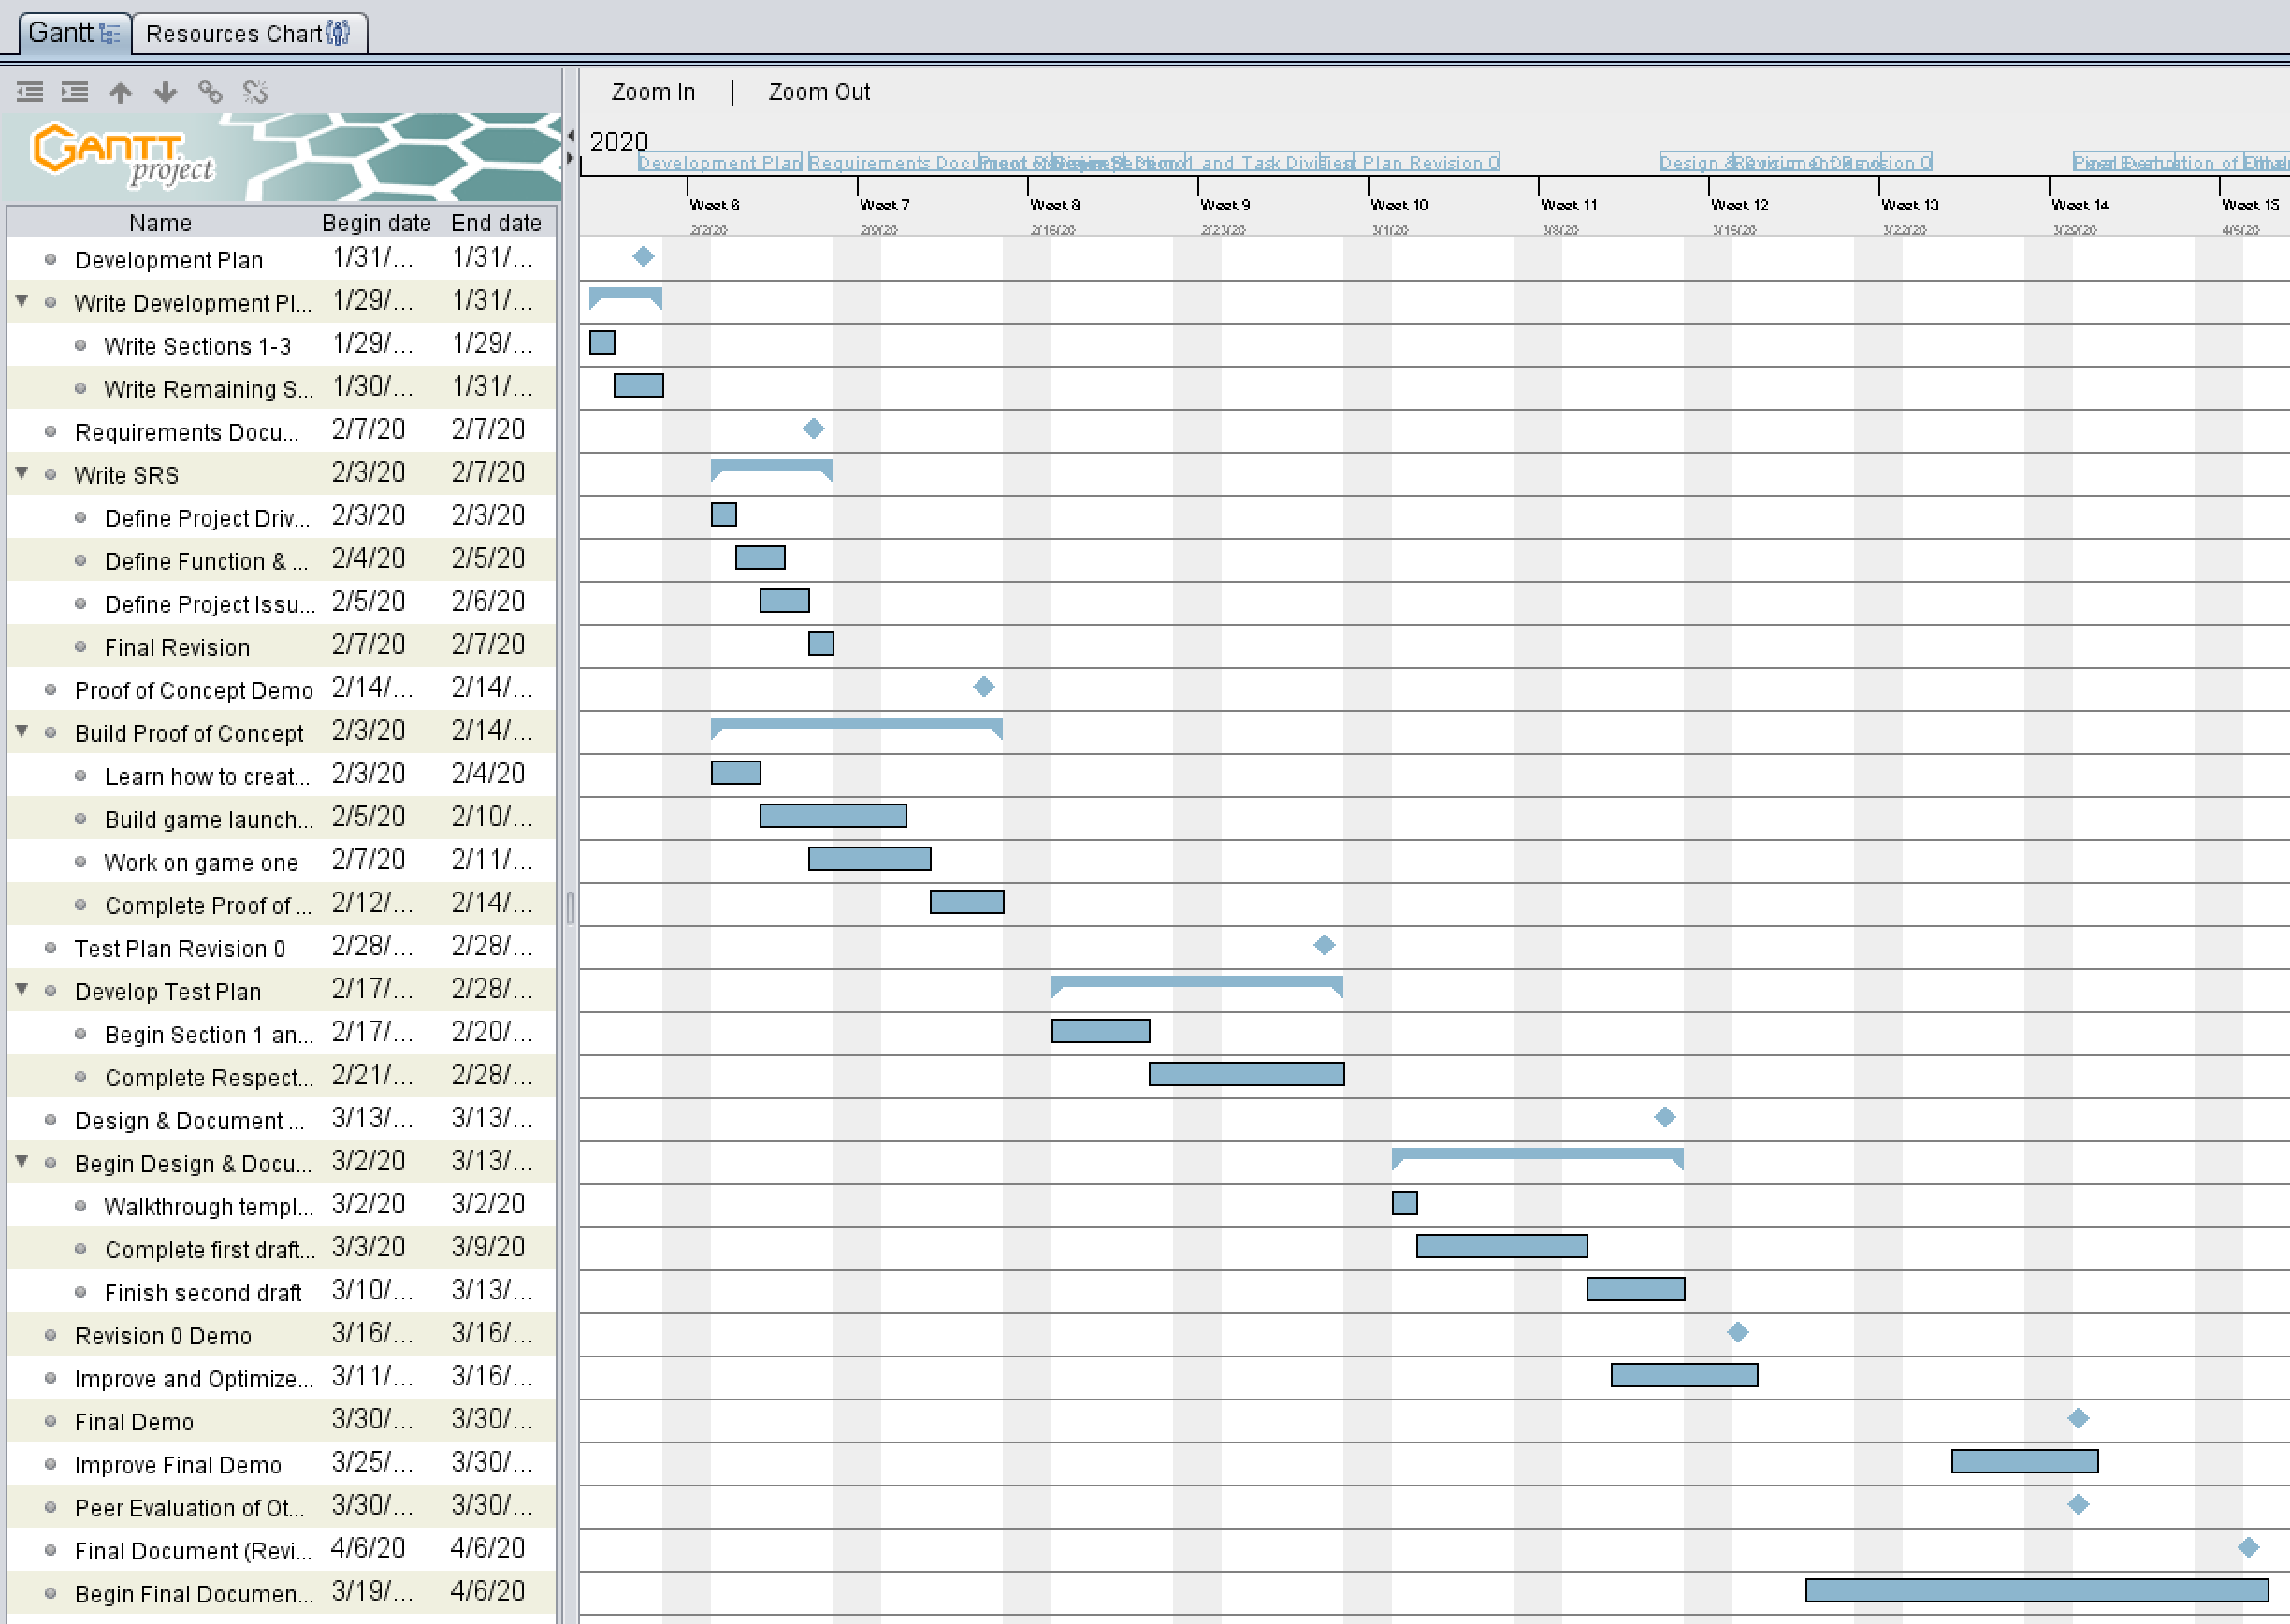
\includegraphics[width=14cm]{TestPlan/GanttRev2.png}\\
%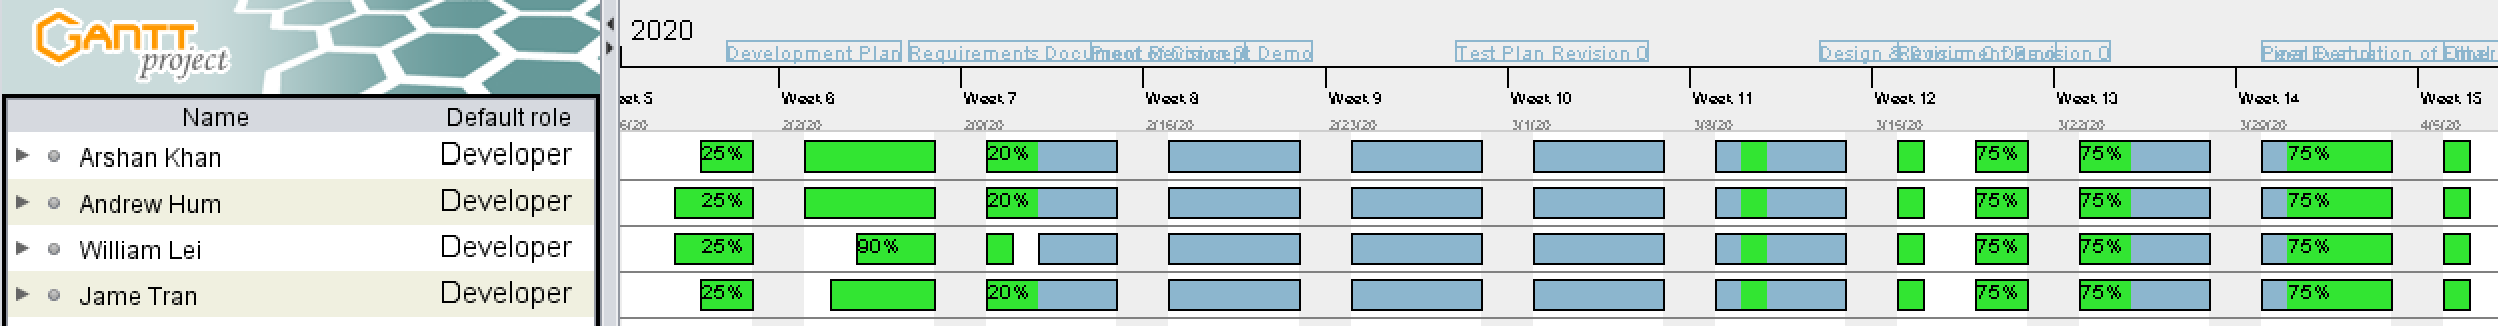
\includegraphics[width=14cm]{TestPlan/GanttRevB2.png}


%\section*{References}

\bibliographystyle {plainnat}
\bibliography {MG}

\end{document}
